\documentclass[11pt,
			   %10pt, 
               %hyperref={colorlinks},
               aspectratio=169,
               hyperref={colorlinks}
               ]{beamer}
\usetheme{Singapore}
\usecolortheme[snowy, cautious]{owl}

\usepackage[utf8]{inputenc}
\usepackage[T1]{fontenc}
\usepackage[american]{babel}
\usepackage{graphicx}
\usepackage{hyperref}
\hypersetup{
    colorlinks=true,
    urlcolor=magenta,
    linkcolor=violet}

\usepackage[natbib=true,style=authoryear,backend=bibtex,useprefix=true]{biblatex}

%\setbeamercolor*{bibliography entry title}{fg=black}
%\setbeamercolor*{bibliography entry location}{fg=black}
%\setbeamercolor*{bibliography entry note}{fg=black}
\definecolor{OwlGreen}{RGB}{75,0,130} % easier to see
\setbeamertemplate{bibliography item}{}
\setbeamerfont{caption}{size=\footnotesize}
\setbeamertemplate{frametitle continuation}{}
\setcounter{tocdepth}{1}
\renewcommand*{\bibfont}{\scriptsize}
\addbibresource{bibliography.bib}

\author{H2O.ai Machine Learning Interpretability Team}
\title{Beyond Reason Codes}
\subtitle{A Bluprint for Human-Centered, Low-Risk AutoML}
\logo{
\includegraphics[height=8pt]{img/h2o_logo.png}}
\institute{\href{https://www.h2o.ai}{H\textsubscript{2}O.ai}}
\date{\today}
\subject{Human-Centered Machine Learning}

\begin{document}
	
	\maketitle
	
	\begin{frame}
	
		\frametitle{Contents}
		
		\tableofcontents{}
		
	\end{frame}

%-------------------------------------------------------------------------------
	\section{Blueprint}
%-------------------------------------------------------------------------------
	
		\begin{frame}
		
			\frametitle{Blueprint}
				
			\begin{figure}[htb]
				\begin{center}
					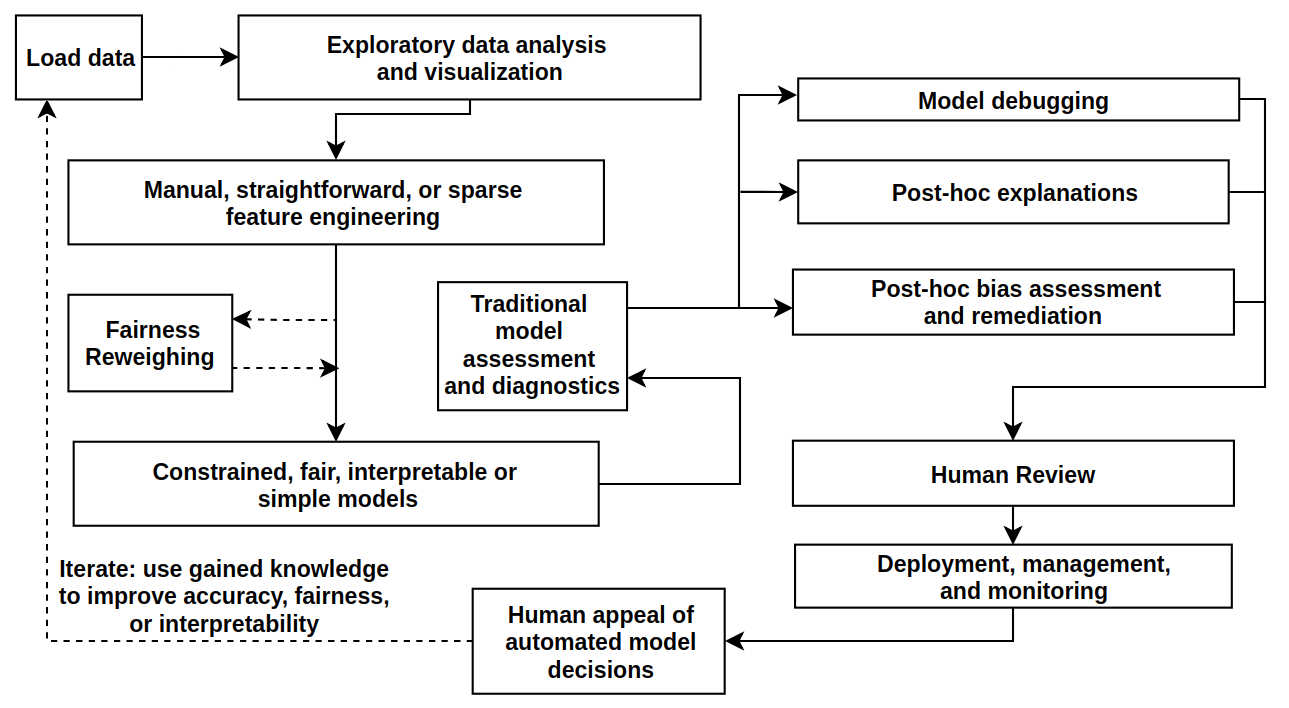
\includegraphics[height=140pt]{img/blueprint.png}
					\label{fig:blueprint}
				\end{center}
			\end{figure}		
		
		\end{frame}


%-------------------------------------------------------------------------------
	\section{EDA}
%-------------------------------------------------------------------------------
	
		\begin{frame}
		
			\frametitle{EDA and Data Visualization}		
			
			\begin{columns}
	
				\column{0.5\linewidth}
				\centering
				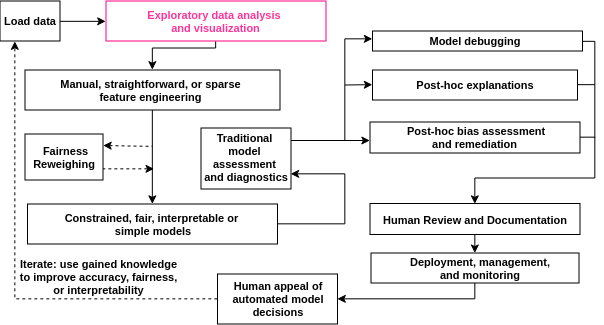
\includegraphics[height=100pt]{img/eda.png}
				
				\column{0.5\linewidth}
				\vspace{-5pt}
				\begin{itemize}
					\item \textbf{Automation} implemented in Driverless AI as AutoViz.
					\item OSS: \href{http://docs.h2o.ai/h2o/latest-stable/h2o-docs/data-science/aggregator.html}{H2O-3 Aggregator}
					\item References: \citefield{wilkinson2018visualizing}{title}; \citefield{wilkinson2006grammar}{title}
				\end{itemize}
				
			\end{columns}
		
		\end{frame}

%-------------------------------------------------------------------------------
	\section{Training}
%-------------------------------------------------------------------------------

%-------------------------------------------------------------------------------
		\subsection{Feature Engineering}
%-------------------------------------------------------------------------------

			\begin{frame}
		
				\frametitle{Manual, Straightforward, or Sparse Feature Engineering}		
		
				\begin{columns}
	
					\column{0.5\linewidth}
					\centering
					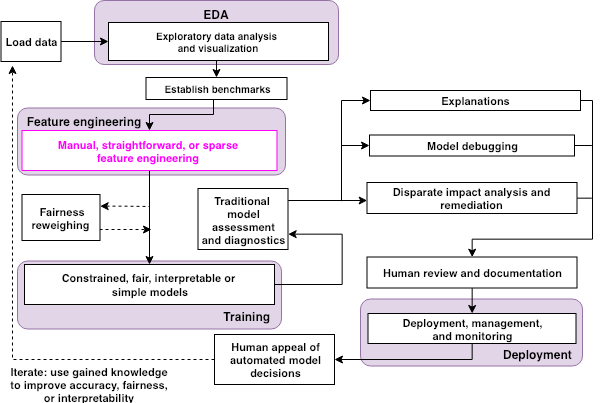
\includegraphics[height=100pt]{img/fe.png}
				
					\column{0.5\linewidth}
					\vspace{-5pt}
					\begin{itemize}
						\item \textbf{Automation} implemented in Driverless AI as high-interpretability transformers.
						\item OSS: \href{https://github.com/pandas-profiling/pandas-profiling}{Pandas Profiler}, \href{https://index.pocketcluster.io/featuretools-featuretools.html}{Feature Tools}
						\item References: \citefield{kanter2015deep}{title}; \citefield{kanter2016label}{title}
					\end{itemize}
				
				\end{columns}		
		
			\end{frame}
	
%-------------------------------------------------------------------------------
		\subsection{Fairness Reweighing}
%-------------------------------------------------------------------------------	
	
			\begin{frame}
		
				\frametitle{Fairness Reweighing}		
			
				\begin{columns}
	
					\column{0.5\linewidth}
					\centering
					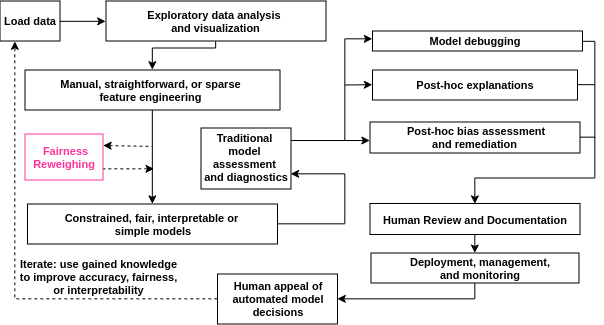
\includegraphics[height=100pt]{img/fr.png}
				
					\column{0.5\linewidth}
					\vspace{-5pt}
					\begin{itemize}
						\item OSS: IBM \href{https://github.com/IBM/AIF360}{AI360}
						\item References: \citefield{calders2010three}{title}; \citefield{kamiran2012data}{title}; \citefield{feldman2015certifying}{title}; \citefield{calmon2017optimized}{title}
						\item \textbf{Roadmap items for MLI-2}.
					\end{itemize}
				
				\end{columns}			
			
			\end{frame}
			
%-------------------------------------------------------------------------------
		\subsection{Interpretable Models}
%-------------------------------------------------------------------------------			
			
			\begin{frame}
		
				\frametitle{Constrained, Fair, Interpretable or Simple Models}		
			
				\begin{columns}
	
					\column{0.5\linewidth}
					\centering
					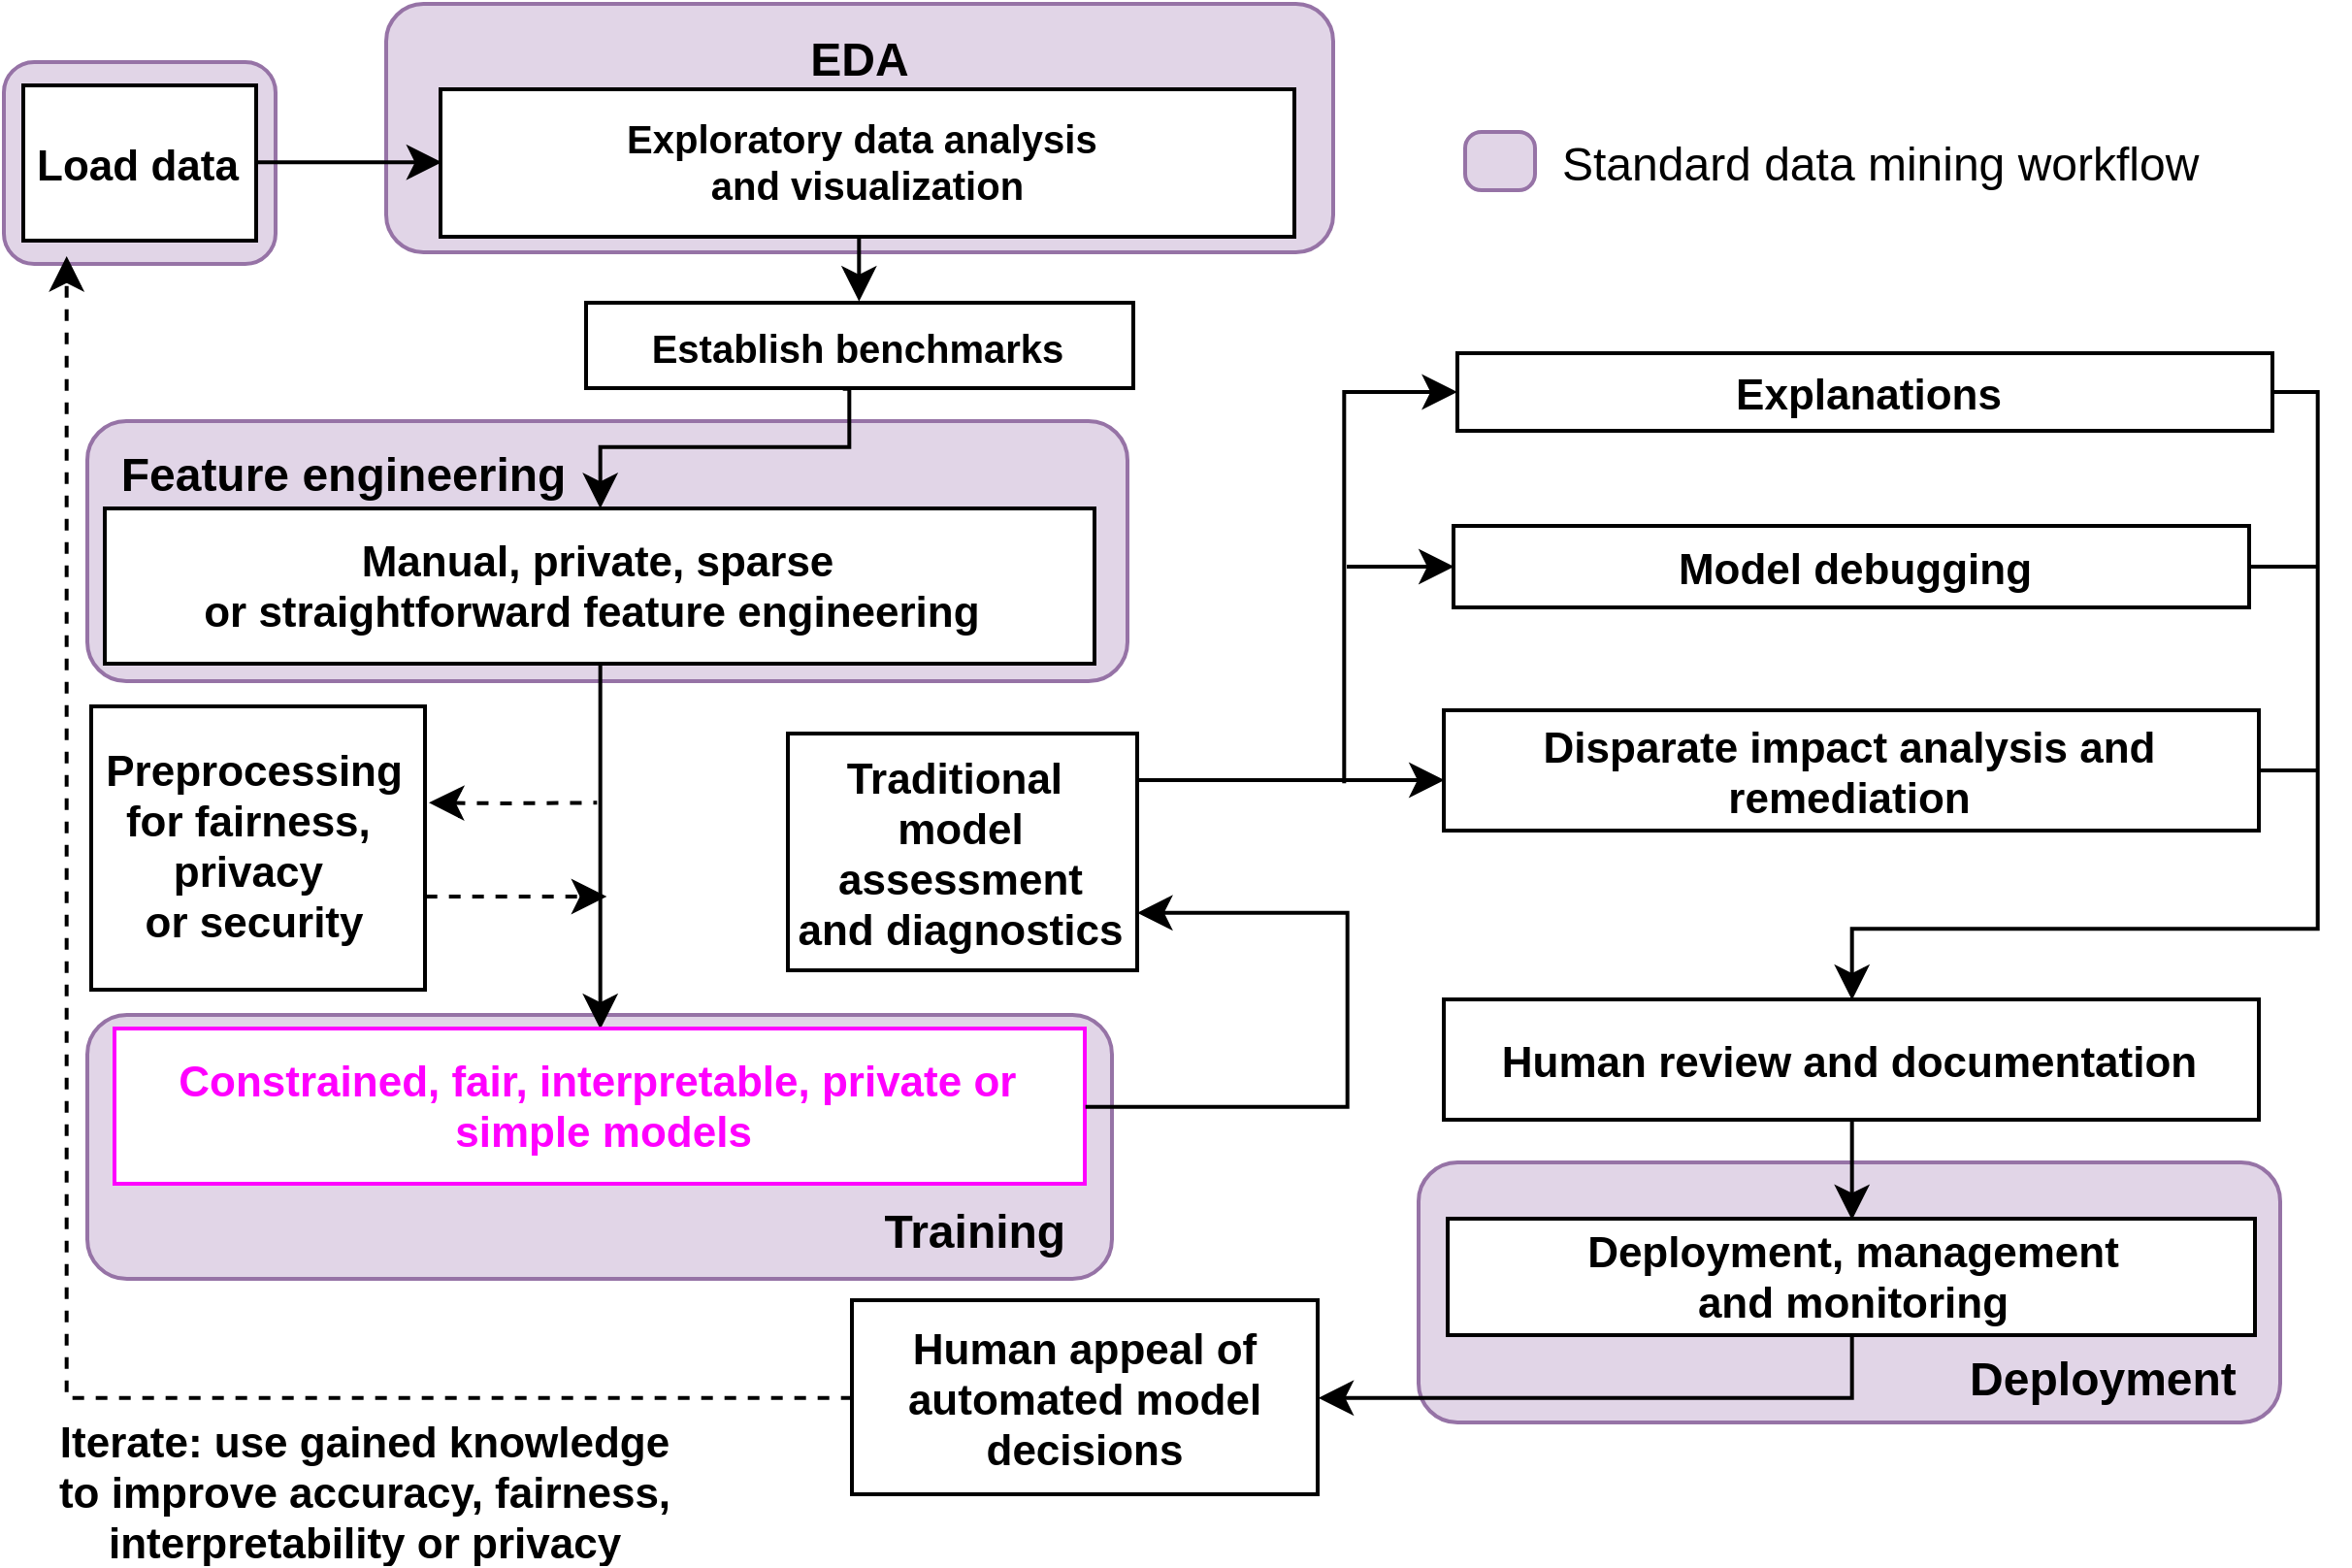
\includegraphics[height=100pt]{img/im.png}
				
					\column{0.5\linewidth}
					\vspace{-5pt}
					\begin{itemize}
						\item \textbf{Automation} implemented in Driverless AI as GLM, RuleFit, Monotonic GBM.
						\item References: \citefield{lime-sup}{title}; \citefield{wf_xnn}{title} (XNN); \citefield{sbrl}{title}	 (SBRL)		
						\item \textbf{LIME-SUP, SBRL, XNN are roadmap items for MLI-2}.
					\end{itemize}
				
				\end{columns}			
			
			\end{frame}

%-------------------------------------------------------------------------------
	\section{Post-Hoc Analysis}
%-------------------------------------------------------------------------------

%-------------------------------------------------------------------------------
		\subsection{Model Assessment}
%-------------------------------------------------------------------------------			

			\begin{frame}
		
				\frametitle{Traditional Model Assessment and Diagnostics}		
			
				\begin{columns}			
			
					\column{0.5\linewidth}
					\centering
					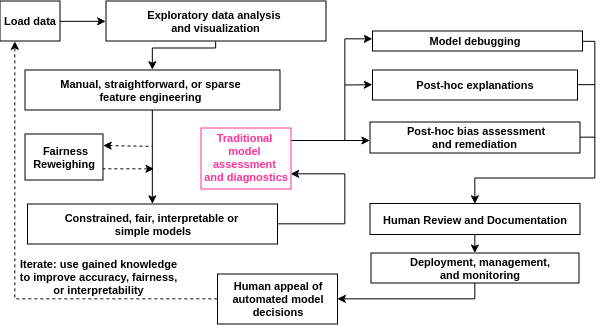
\includegraphics[height=100pt]{img/ma.png}
				
					\column{0.5\linewidth}
					\vspace{-5pt}
					\begin{itemize}
						\item Residual analysis, Q-Q plots, AUC and lift curves confirm model is accurate and meets assumption criteria.
						\item Implemented as model diagnostics in Driverless AI.
						\item \textbf{Residual analysis is roadmap item for model diagnostics in Driverless AI}.
					\end{itemize}
				
				\end{columns}
		
			\end{frame}

%-------------------------------------------------------------------------------
		\subsection{Model Debugging}
%-------------------------------------------------------------------------------	

			\begin{frame}
		
				\frametitle{Model Debugging}		
			
				\begin{columns}
	
					\column{0.5\linewidth}
					\centering
					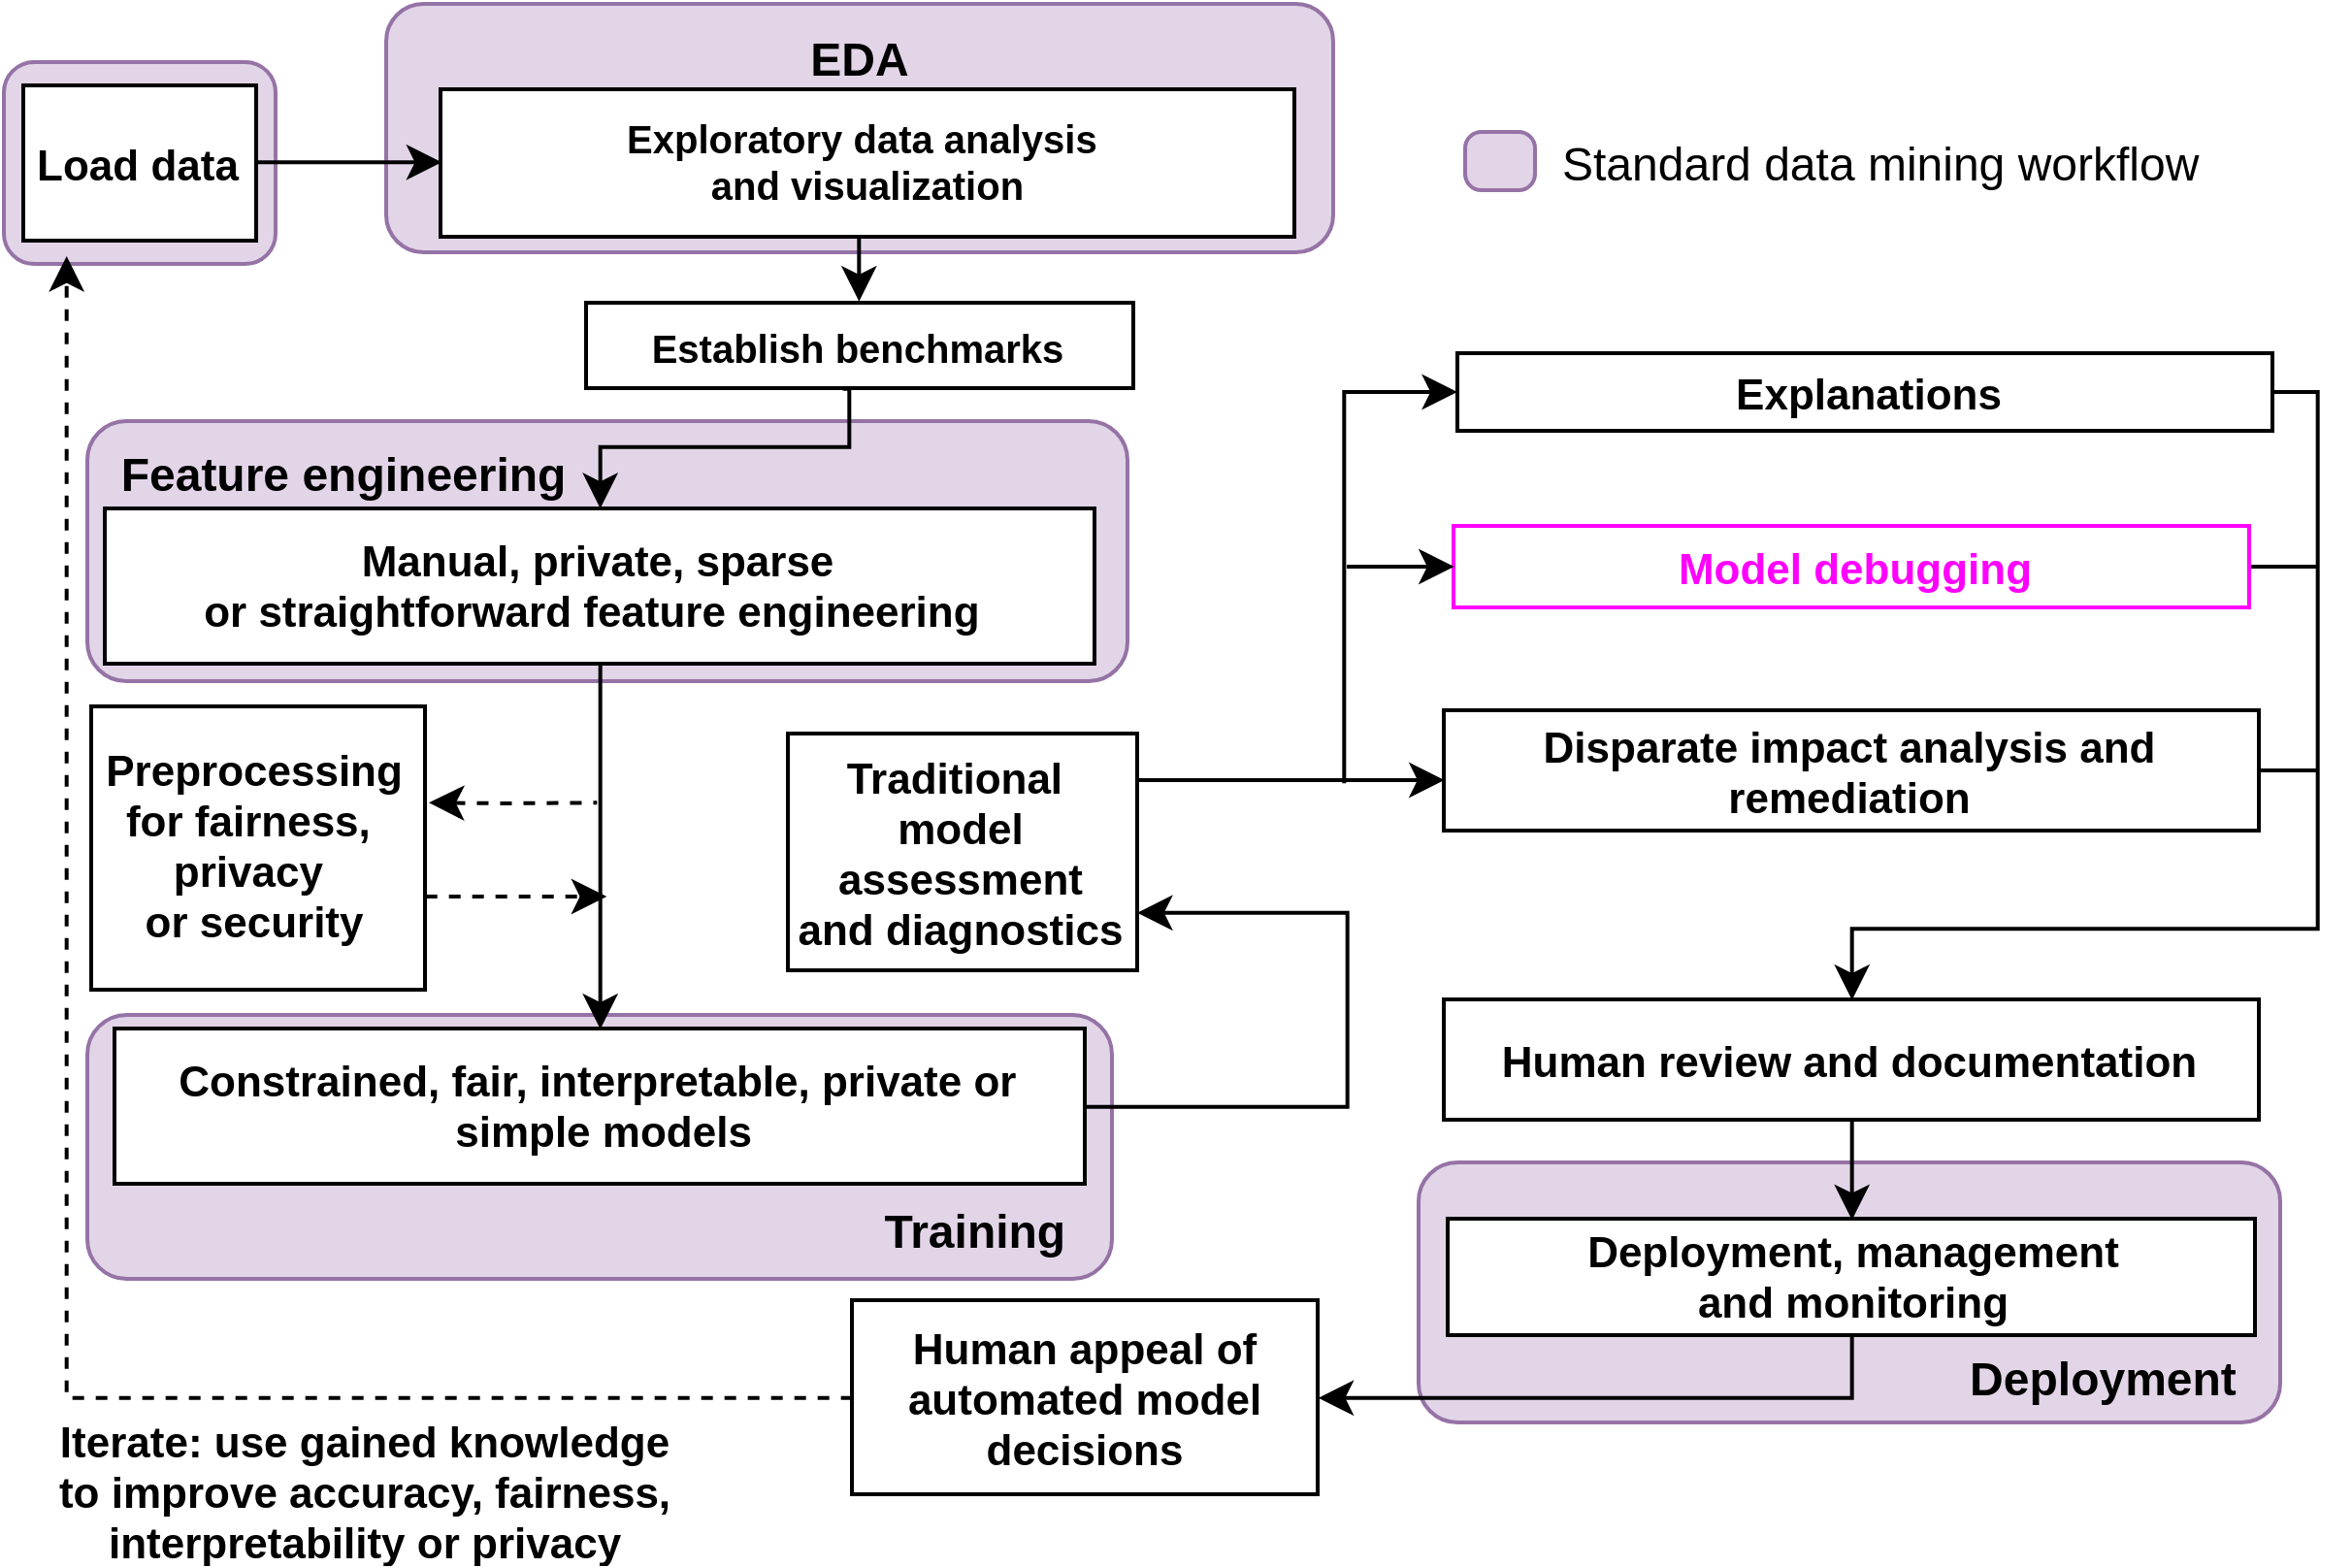
\includegraphics[height=100pt]{img/md.png}
				
					\column{0.5\linewidth}
					\vspace{-5pt}
					\begin{itemize}
						\item Understanding and eliminating errors in model predictions by model testing: adversarial examples, "what-if" analysis, random attacks, explanation of residuals.
						\item OSS: \href{https://github.com/tensorflow/cleverhans}{cleverhans}, \href{https://github.com/SauceCat/PDPbox}{pdpbox}, \href{https://pair-code.github.io/what-if-tool/index.html}{what-if tool}
						\item \textbf{Adversarial examples, "what-if" analysis, explanation of residuals, measures of epistemic uncertainty are implemented and roadmap items in MLI-2.}
					
					\end{itemize}
				
				\end{columns}			
			
			\end{frame}
			
%-------------------------------------------------------------------------------
		\subsection{Post-hoc Explanations}
%-------------------------------------------------------------------------------			
			
			\begin{frame}
		
				\frametitle{Post-hoc Explanations}		
			
				\begin{columns}
	
					\column{0.5\linewidth}
					\centering
					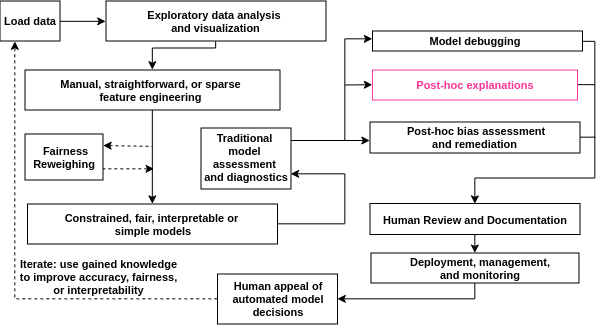
\includegraphics[height=100pt]{img/exp.png}
				
					\column{0.5\linewidth}
					\vspace{-5pt}
					\begin{itemize}
						\item LIME and Tree SHAP implemented Driverless AI.
						\item OSS: \href{https://github.com/marcotcr/lime}{lime}, \href{https://github.com/slundberg/shap}{shap} 
						\item References: \citefield{lime}{title}; \citefield{shapley}{title}; \citefield{please_stop}{title} (criticism)
						\item Tree SHAP is roadmap item for H2O-3; \textbf{Explanations for unstructured data are roadmap for MLI-2}.
					\end{itemize}
				
				\end{columns}
		
			\end{frame}

			\begin{frame}
		
				\frametitle{Interlude: The Time--Tested Shapley Value}		
			
				\begin{enumerate}
				
					\item \textbf{In the beginning}: \citefield{shapley1953value}{title}, \citefield{shapley1953value}{year}
					\item \textbf{Nobel-worthy contributions}: \citefield{shapley1988shapley}{title}, \citefield{shapley1988shapley}{year}
					\item \textbf{Shapley regression}: \citefield{lipovetsky2001analysis}{title}, \citefield{lipovetsky2001analysis}{year}
					\item \textbf{First reference in ML?} \citefield{keinan2004fair}{title}, \citefield{keinan2004fair}{year} 	
					\item \textbf{Into the ML research mainstream, i.e. JMLR}: \citefield{kononenko2010efficient}{title}, \citefield{kononenko2010efficient}{year}
					\item \textbf{Into the real-world data mining workflow ... \textit{finally}}: \citefield{tree_shap}{title}, \citefield{tree_shap}{year}	
					\item \textbf{Unification}: \citefield{shapley}{title}, \citefield{shapley}{year}	
				
				\end{enumerate}
			
			\end{frame}
			
%-------------------------------------------------------------------------------
		\subsection{Post-hoc Disparate Impact Remediation}
%-------------------------------------------------------------------------------					
		
			\begin{frame}		
		
			\frametitle{Post-hoc Disparate Impact Assessment and Remediation}		
			
			\begin{columns}
	
				\column{0.5\linewidth}
				\centering
				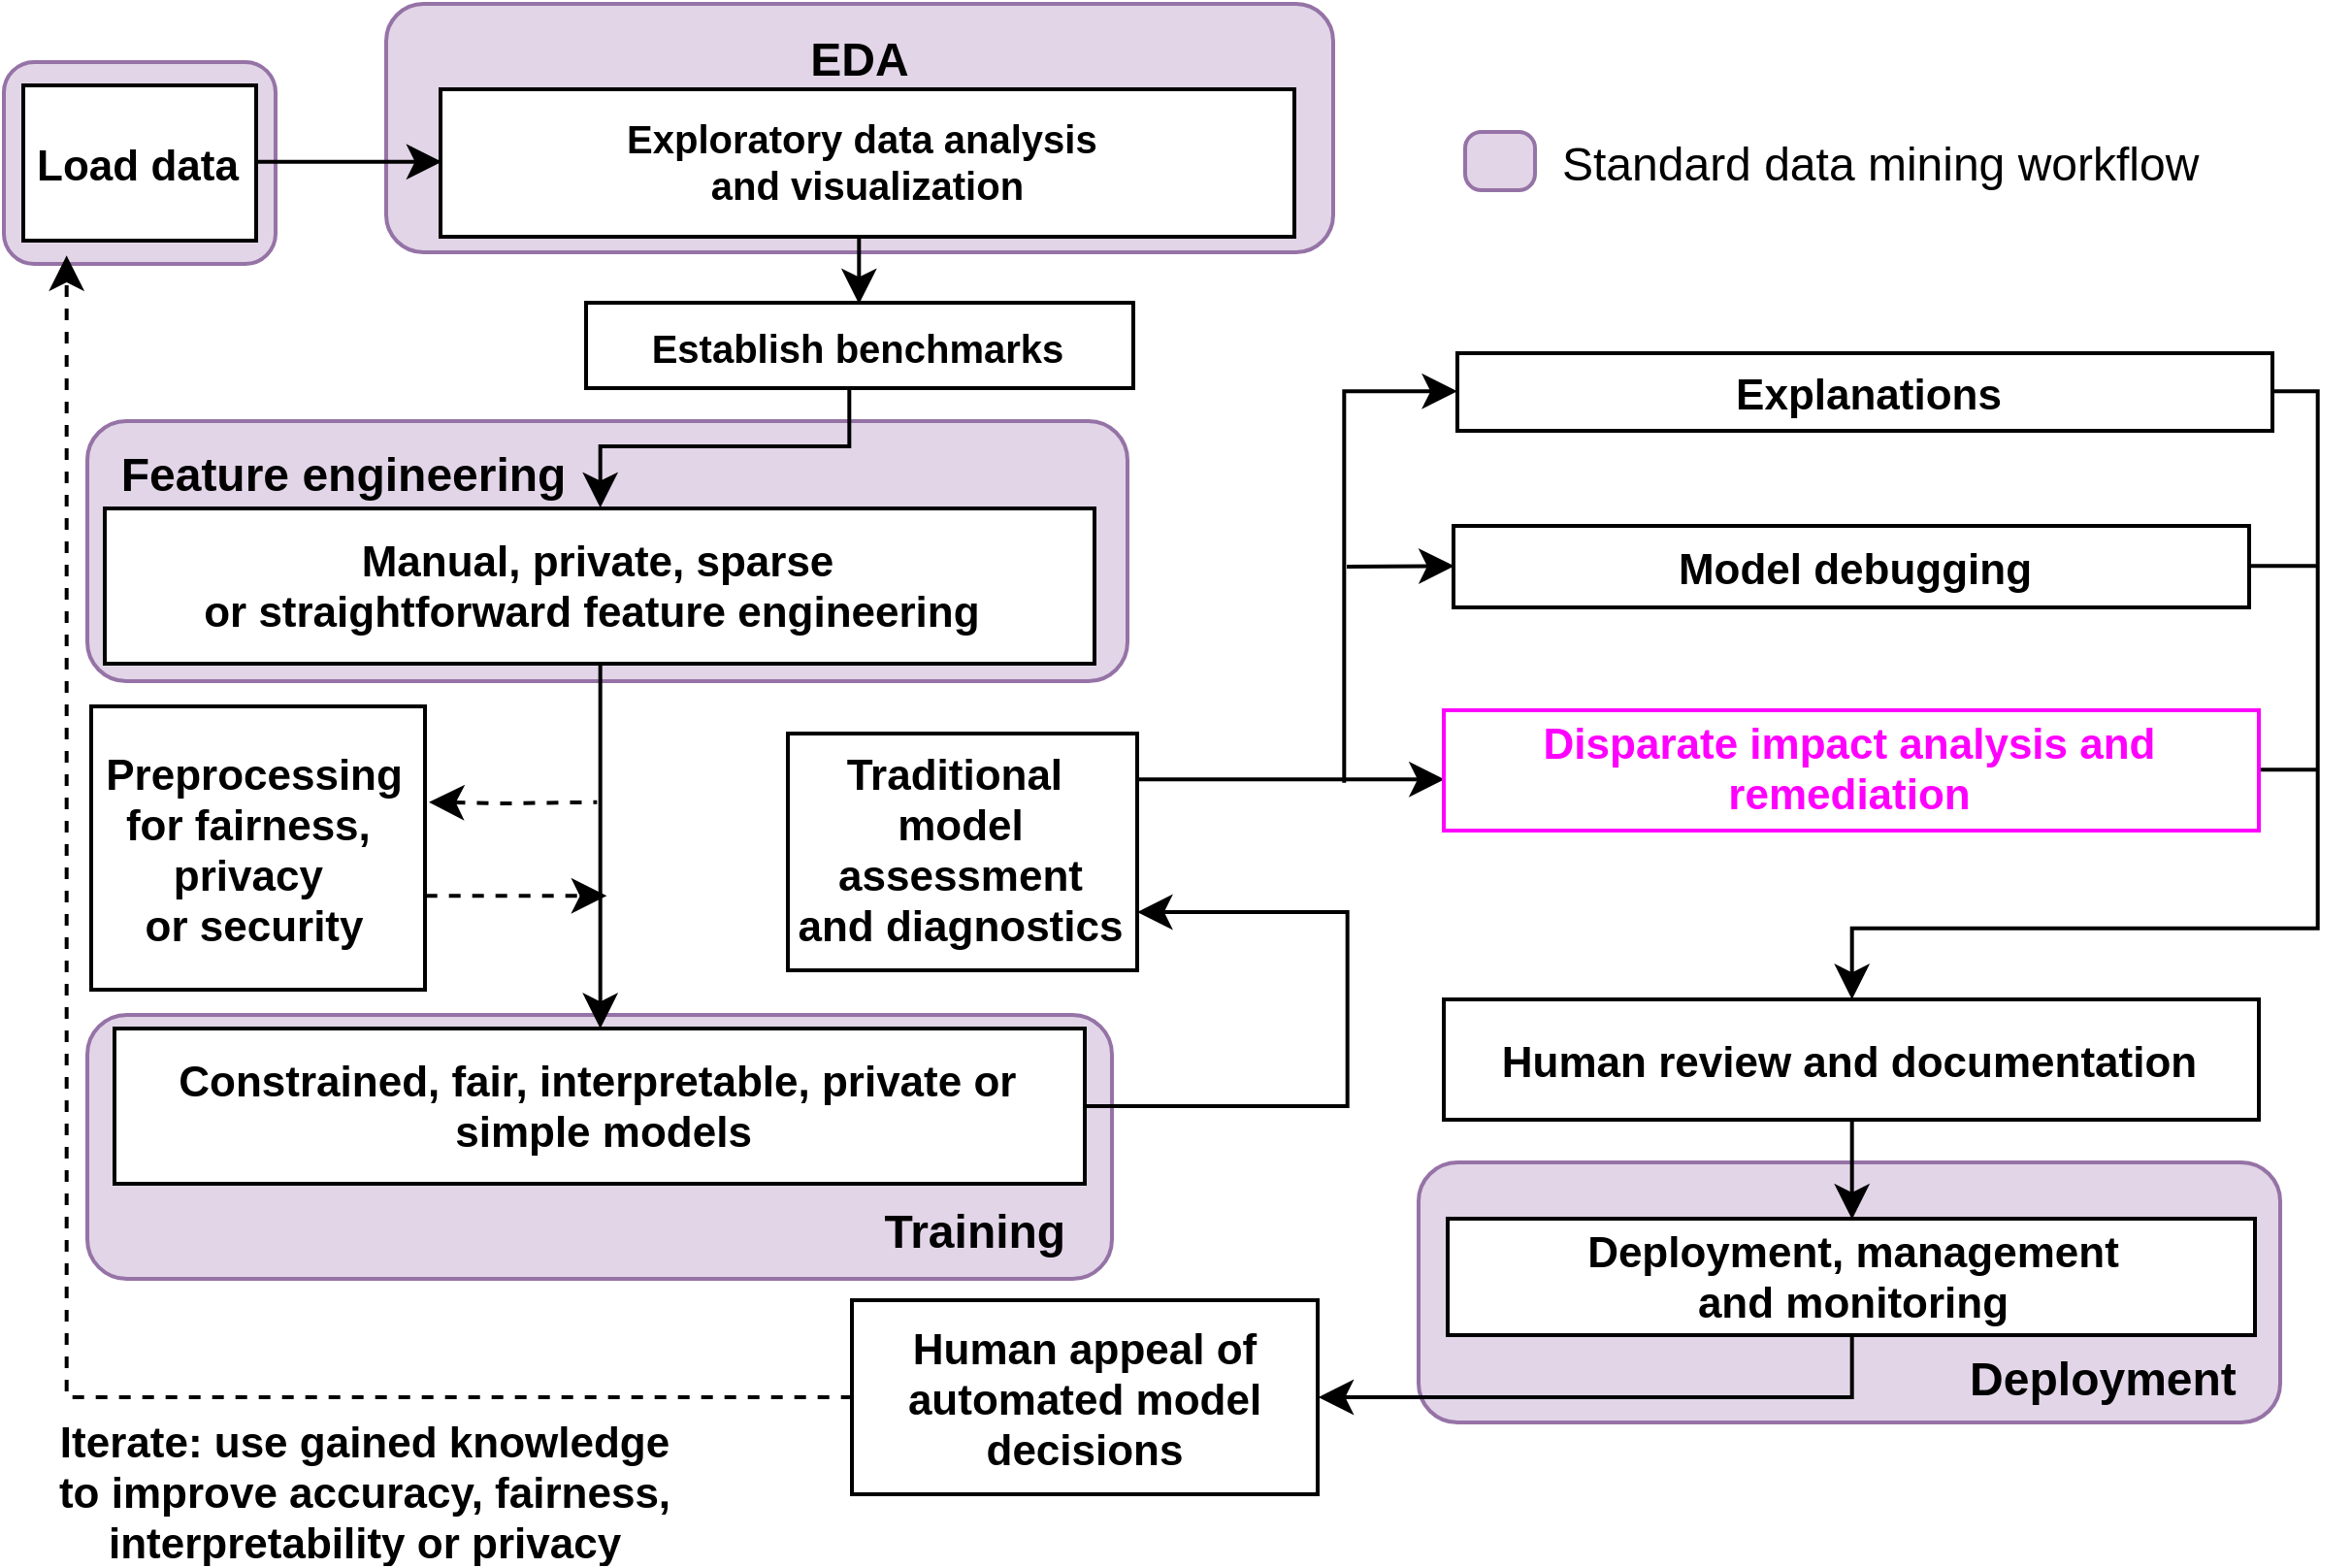
\includegraphics[height=100pt]{img/fair.png}
				
				\column{0.5\linewidth}
				\vspace{-5pt}
				\begin{itemize}
					\item Disparate impact analysis can be performed manually using Driverless AI or H2O-3.
					\item OSS: \href{https://github.com/dssg/aequitas}{aequitas}, IBM \href{https://github.com/IBM/AIF360}{AI360}, \href{https://github.com/LASER-UMASS/Themis}{themis}
					\item References: \citefield{hardt2016equality}{title}; \citefield{feldman2015certifying}{title} 
					\item \textbf{Disparate impact analysis and remediation are roadmap items for MLI-2.}
				\end{itemize}
				
			\end{columns}
		
		\end{frame}



%-------------------------------------------------------------------------------
	\section{Human Review}
%-------------------------------------------------------------------------------

		\begin{frame}
		
			\frametitle{Human Review and Documentation}		
			
			\begin{columns}
	
				\column{0.5\linewidth}
				\centering
				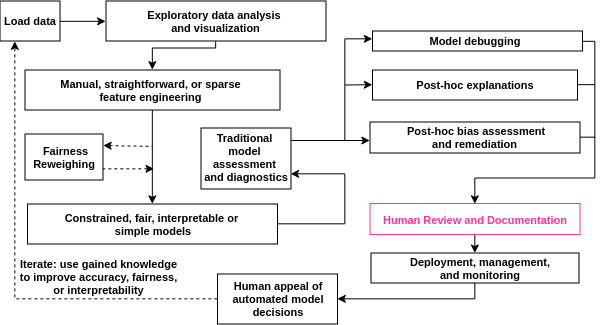
\includegraphics[height=100pt]{img/hr.png}
				
				\column{0.5\linewidth}
				\vspace{-5pt}
				\begin{itemize}
					\item Implemented as AutoDoc in\\ Driverless AI.
					\item \textbf{Various interpretability and fairness roadmap items to be added to AutoDoc}.
				\end{itemize}
				
			\end{columns}
		
		\end{frame}

%-------------------------------------------------------------------------------
	\section{Deployment}
%-------------------------------------------------------------------------------

		\begin{frame}

			\frametitle{Deployment, Management, and Monitoring}		
			
			\begin{columns}
	
				\column{0.5\linewidth}
				\centering
				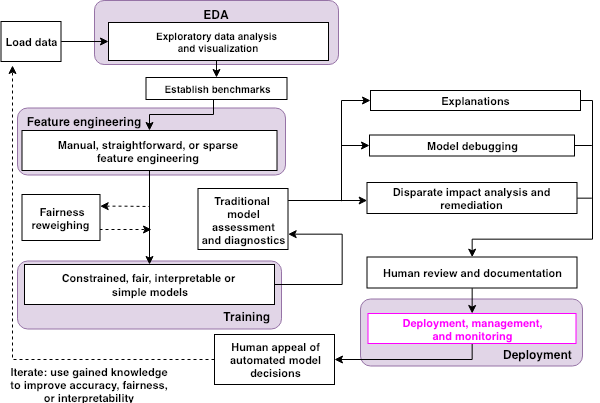
\includegraphics[height=100pt]{img/deploy.png}
				
				\column{0.5\linewidth}
				\vspace{-5pt}
				\begin{itemize}
					\item Monitor models for accuracy and fairness in real-time, track model and data lineage.
					\item OSS: \href{https://github.com/mlflow/mlflow}{mlflow}, \href{https://github.com/mitdbg/modeldb}{modeldb}
					\item Reference: \citefield{vartak2016m}{title}
					\item \textbf{Broader roadmap item for H2O.ai}.
				\end{itemize}
				
			\end{columns}
		
		\end{frame}

%-------------------------------------------------------------------------------
	\section{Human Appeal}
%-------------------------------------------------------------------------------

		\begin{frame}	
			\frametitle{Iterate: Use Gained Knowledge to Improve Accuracy, Fairness, or Interpretability}		
			
			\begin{figure}[htb]
				\begin{center}
					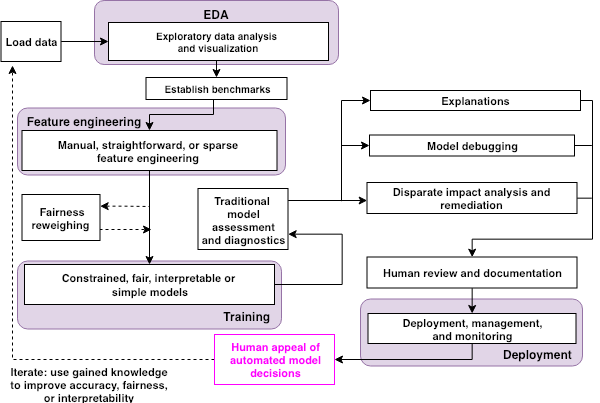
\includegraphics[height=120pt]{img/ha.png}
					\label{fig:blueprint}
				\end{center}
			\end{figure}	

			\centering
			\vspace{-10pt}
			\textit{Very} important, may require custom implementation for each deployment environment?

		\end{frame}

%-------------------------------------------------------------------------------
	\section{Iterate}
%-------------------------------------------------------------------------------

		\begin{frame}	

			\frametitle{Iterate: Use Gained Knowledge to Improve Accuracy, Fairness, or Interpretability}		
			
			\begin{figure}[htb]
				\begin{center}
					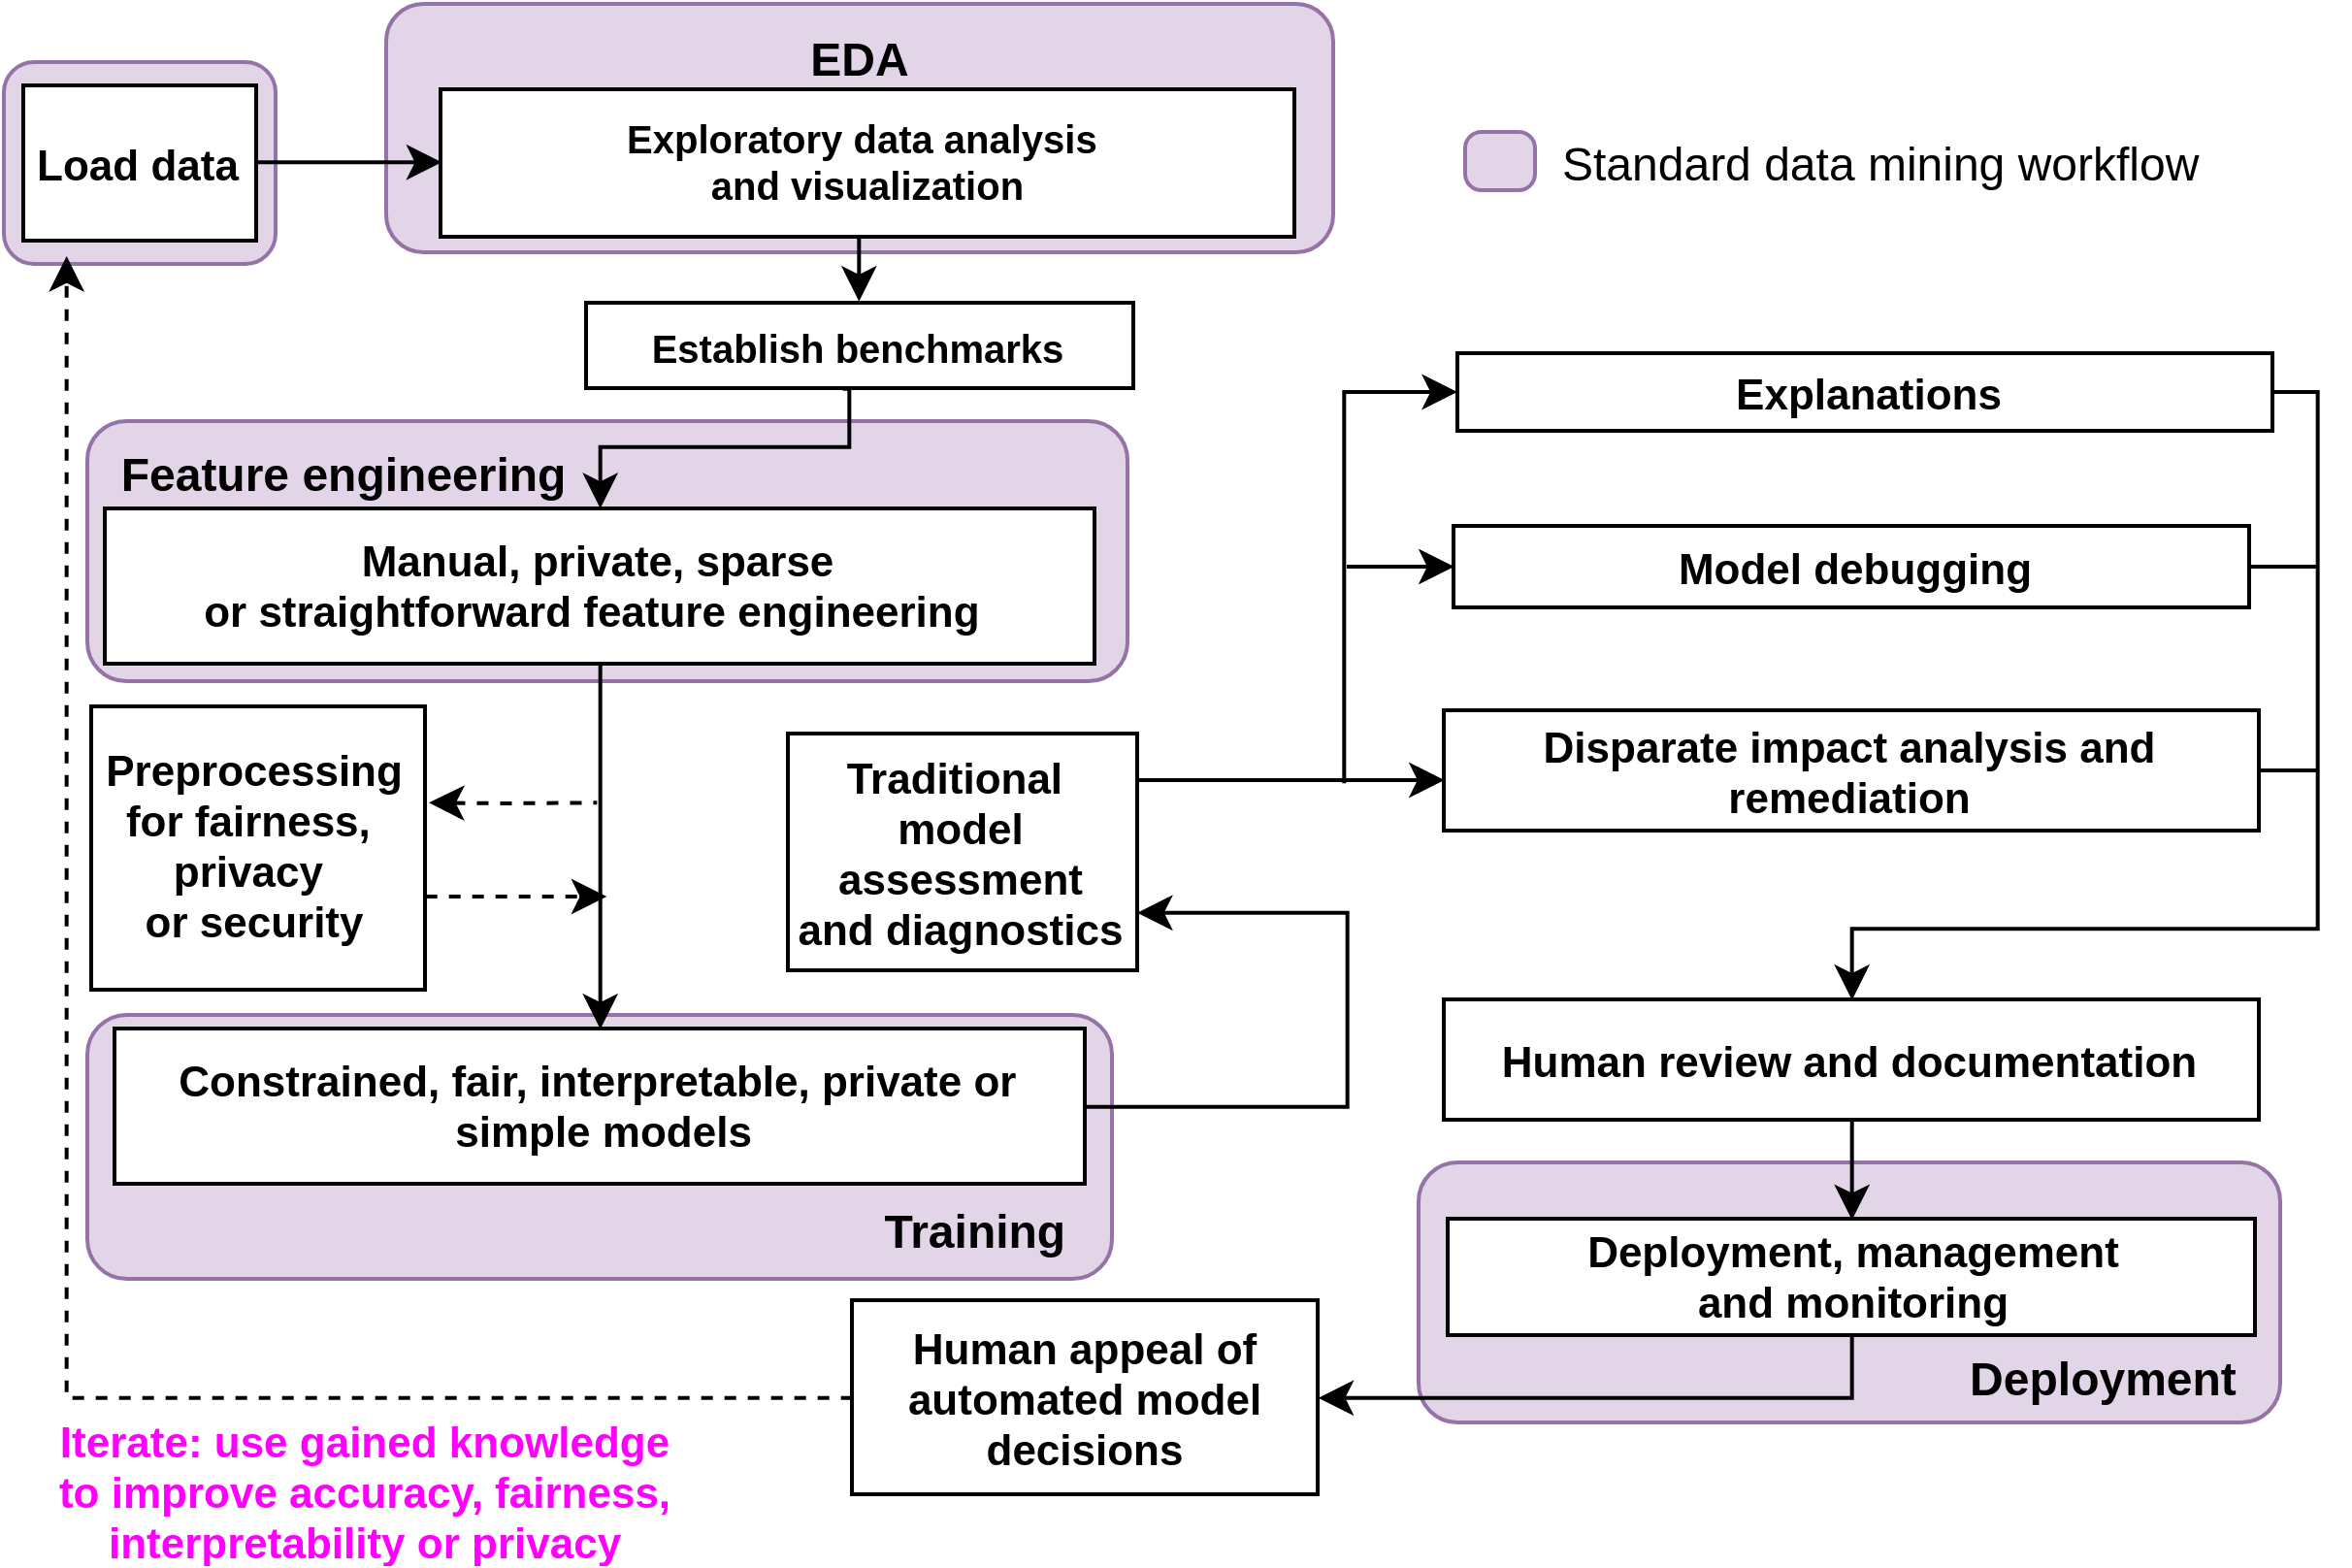
\includegraphics[height=120pt]{img/iter.png}
					\label{fig:blueprint}
				\end{center}
			\end{figure}	

			\centering
			
			Improvements, KPIs should not be restricted to accuracy alone.
		
		\end{frame}

%-------------------------------------------------------------------------------
	\section{Open Questions}
%------------------------------------------------------------------------------

		\begin{frame}

			\frametitle{Open Conceptual Questions}		

			\begin{itemize}
				\item How much automation is appropriate, 100\%?
				\item How to automate learning by iteration, reinforcement learning?
				\item How to implement human appeals, is it productizable?
			\end{itemize}
			
		\end{frame}

%-------------------------------------------------------------------------------
%	References
%-------------------------------------------------------------------------------

	\begin{frame}[t, allowframebreaks]
	
		\frametitle{References}
		
			\vspace{10pt}		
		
			\textbf{Driverless AI API Interpretability Technique Examples:}\\
			\small{\url{https://github.com/h2oai/driverlessai-tutorials}}
			
			\vspace{10pt}		
		
		
			\textbf{In-Depth Open Source Interpretability Technique Examples:}\\
			\small{\url{https://github.com/jphall663/interpretable_machine_learning_with_python}}
			
			\vspace{10pt}
			
			\textbf{"Awesome" Machine Learning Interpretability Resource List:}\\
			\small{\url{https://github.com/jphall663/awesome-machine-learning-interpretability}}
			
		
		\framebreak		
		
		\printbibliography
		
	\end{frame}

\end{document}